\chapterimage{head2.png} % Chapter heading image
\chapter{Double Well}
\section{Building double well by analytical form}
\subsection{Analytical form of potential}
\begin{align}
        V(x) &= -\frac{1}{4} h^4 x^2 + \frac{1}{2} c^2 x^4 + d\\
        c    &= \sqrt{\frac{2H}{W^4}},H > 0 \\
        h    &= \sqrt{2Wc} \\
        F(x) &= \frac{1}{2} h^4 x - 2 c^2 x^3\\
        p_{\rm eq}(x) &= \exp{(-V(x))} \\
        D &= 4.845 \times 10^{9}~~\text{\AA}^2~s^{-1}\\
\end{align}
where $d$ is y-intercept, $H$ is the height of the central peak, and $W$ is the width between two valleys. In the following case, $H=5$ and $W=10$.
\begin{center}
        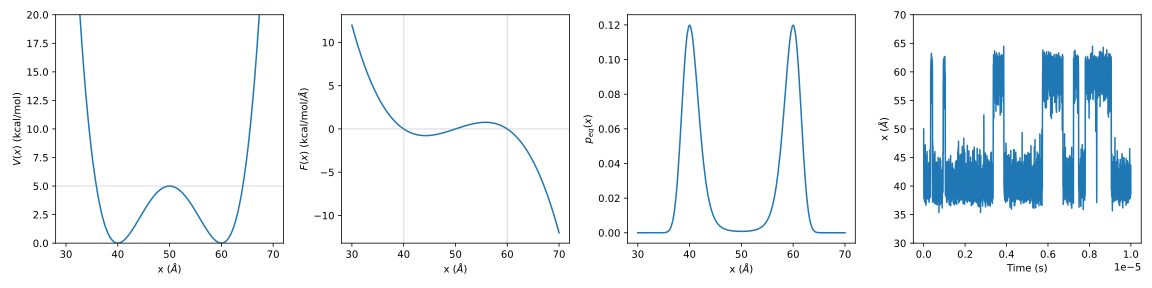
\includegraphics[scale=0.35]{ch1/double_well.pdf} 
\end{center}
\subsection{Eigenvector}
All eigenvectors are shown. As you can see, there are numerical instabilities.
\begin{center}
        \includegraphics[scale=0.25]{ch5/eigv_1_24.png} 
\end{center}
\begin{center}
        \includegraphics[scale=0.25]{ch5/eigv_25_48.png} 
\end{center}
\begin{center}
        \includegraphics[scale=0.25]{ch5/eigv_49_72.png} 
\end{center}

\section{Diagonalization of the operator}
\begin{definition}[Basis functions]
\begin{align}
        \psi^0_i(x) &= \rho_{\rm eq}(x) \phi^0_i(x) \\
        \phi^0_i(x) &= \sum_n c^0_n u_n(x).
\end{align}
\label{basisfunctions}
\end{definition}

\begin{definition}[Eigenvector matrix]
\begin{equation}
\Psi=
\begin{bmatrix}
\vert & \vert &  & \vert \\
\psi_1(x) & \psi_2(x) & \cdots & \psi_{N_v}(x) \\
\vert & \vert &  & \vert 
\end{bmatrix}
\end{equation}
\label{eigenvectormatrix}
Here, we get a set of orthonormal basis, $\langle \psi_i |$. The left part in the following part is 
\begin{equation}
        \Psi^T_{72\times 193}\Psi_{193 \times 72} = (\Psi^T\Psi)_{72 \times 72}
\end{equation}
The completeness relationship should satisfy the following
\begin{equation}
        \langle \psi_i(x),\psi_i(x)\rangle _{w} = \sum_{j=1}^{193}w(x_j)\psi_i(x_j)\psi_i(x_j)  = 1
\end{equation}
\begin{center}
        \includegraphics[scale=0.4]{ch5/eigenvec_matrix_complete.png}   
\end{center}
But the result does not follow that, implying our eigenvectors from sFEM can not be a basis set.
\end{definition}

\section{Forward algorithm}
\subsection{Probability Meaning}
$ \left<\alpha_{t_{\tau}}|x \right>$ is the joint probability amplitude of emitting a partial sequence of outputs $(y_1,\cdots,y_{\tau})$ and ending up in state $x_{\tau}$. That is,
\begin{equation}
        (\left<\alpha_{t_{\tau}}|x \right>)^2 = p(y_1,\cdots,y_{\tau}, x_{\tau})
\end{equation}
For example, $(\left<\alpha_{t_2}|x \right>)^2 = p(y_1, y_2, x_2)$
\begin{center}
        \includegraphics[scale=0.8]{ch2/alpha_example.pdf}
\end{center}
\subsection{alpha-t0}
\begin{definition}[$\left< \hat{\alpha}_{t_0} \right|$]
Since there is no external forces, the initial state, $\left< \alpha_{t_0} \right|$, is assumed to follow the equilibrium distribution $\rho_{eq}(x)=\sqrt{p_{eq}(x)}$, that is
\begin{equation}
        \left< \alpha_{t_0} | x \right> = \rho_{eq}(x)
\end{equation}
\begin{center}
        \includegraphics[scale=0.45]{ch5/alpha_t0.png}   
\end{center}
And we know
\begin{align*}
        p(x,t=0) &= \rho_{eq}(x) \rho_{eq}(x)\\
        &= \rho_{eq}(x)[\left< \alpha_{t_0} | \psi_1 \right> \psi_1(x) + \left< \alpha_{t_0} | \psi_2 \right>\psi_2(x)+\cdots+\left< \alpha_{t_0} | \psi_{72} \right>\psi_{72}(x)]       
\end{align*}
where
\begin{align*}
        \left< \alpha_{t_0} | \psi_j \right> = \int w(x) \rho_{eq}(x) \psi_j(x) dx \approx \sum_{i=1}^{193} w(x_i) \rho_{eq}(x_i) \psi_j(x_i)
\end{align*}
$\left< \alpha_{t_0} \right|$ is a vector, which is shown in the right-bottom figure.
\begin{equation}
        \left< \alpha_{t_0} \right| = \begin{bmatrix}\left< \alpha_{t_0} | \psi_1 \right> & \left< \alpha_{t_0} | \psi_2 \right> & \cdots & \left< \alpha_{t_0} | \psi_{72} \right> \end{bmatrix}
\end{equation}
and the norm of $\left< \alpha_{t_0} \right|$ is defined by
\begin{align}
        \norm{\alpha_{t_0}} &=  \sqrt{\int w(x) (\left< \alpha_{t_0} | x_i \right>)^2 dx} \approx \sqrt{ \sum_{i=1}^{193} w(x_i) (\left< \alpha_{t_0} | x_i \right>)^2 } \\
        \norm{\alpha_{t_0}} &= \sqrt{(\left< \alpha_{t_0} | \psi_1 \right>)^2 + (\left< \alpha_{t_0} | \psi_2 \right>)^2 +\cdots + (\left< \alpha_{t_0} | \psi_{72} \right>)^2}
\end{align}
Furthermore, note that
\begin{equation}
        \left< \hat{\alpha}_{t_0} \right| = \frac{\left< \alpha_{t_{0}} \right|}{\norm{\alpha_{t_{0}}}} = \left< \alpha_{t_{0}} \right|
\end{equation}
because $\norm{\alpha_{t_0}} = 1$
\end{definition}

\begin{definition}[$\rho(x, t=\Delta t) = \left<\alpha_{t_0}| e^{-\textbf{H}\Delta t}|x \right>$]
\begin{align*}
        &p(x,t=\Delta t) = \rho_{eq}(x) \rho(x, \Delta t)\\
        &= \rho_{eq}(x)[ \left< \alpha_{t_0} | \psi_1 \right> e^{-\lambda_{1}\Delta t}\psi_1(x) + \cdots+ \left< \alpha_{t_0} | \psi_{72} \right> e^{(-\lambda_{72}\Delta t)}\psi_{72}(x)]  \\
        &=  \rho_{eq}(x)[ \left< \alpha_{t_0} | \psi_1 \right>\psi_1(x)+ \cdots + \left< \alpha_{t_0} | \psi_{72} \right> e^{(-\lambda_{72}\Delta t)}\psi_{72}(x)]  
\end{align*}
where $\lambda_1 = 0$
\begin{center}
        \includegraphics[scale=0.35]{ch5/alpha_t0_exp_dt.png}   
\end{center}
\end{definition}

\subsection{alpha-t1}
\begin{definition}[$\left< \hat{\alpha}_{t_1}\right|$]
\begin{equation}
        \left< \alpha_{t_1} \right| = \left< \alpha_{t_0} \right| e^{-\textbf{H} \Delta t} \textbf{y}_1     
\end{equation}
\begin{center}
        \includegraphics[scale=0.25]{ch5/photon_operator_y1.png}   
\end{center}
$\left< \alpha_{t_1} \right|$ carries "the joint probability amplitude" of observing all the photon data during $[0, t_1]$ and the system state at $t_1$, that is
\begin{equation}
        p(x, y_1) = (\left< \alpha_{t_1} | x \right>)^2
\end{equation}
We can do normalization to get $\left< \hat{\alpha}_{t_1} \right|$.
\begin{equation}
        \left< \hat{\alpha}_{t_1} \right| = \frac{\left< \alpha_{t_0} \right| e^{-\textbf{H}\Delta t} \textbf{y}_1}{\norm{\left< \alpha_{t_0} \right| e^{-\textbf{H}\Delta t} \textbf{y}_1}} = \frac{\left< \alpha_{t_{1}} \right|}{\norm{\alpha_{t_{1}}}}
\end{equation}
\begin{center}
        \includegraphics[scale=0.4]{ch5/alpha_1.png}   
\end{center}
$\left< \hat{\alpha}_{t_1} \right|$ is a probability amplitude, which square is 
\begin{align*}
        p(x | y_1) =  (\left< \hat{\alpha}_{t_1} | x \right>)^2
\end{align*}
Therefore
\begin{align*}
        \int p(x|y_1) dx \approx \sum_{k=1}^{193}w(x_k)(\left< \hat{\alpha}_{t_1} | x_k \right>)^2 &= 1 \\
        \norm{\hat{\alpha_{t_1}}} &= 1
\end{align*}
\end{definition}

\begin{definition}[$\left< \hat{\alpha}_{t_1}| e^{-\textbf{H}\Delta t} \right|$]
\begin{align*}
        \left< \hat{\alpha}_{t_1}| e^{-\textbf{H}\Delta t} \right| &= 
        \begin{bmatrix}
                \left< \hat{\alpha}_{t_1}| e^{-\textbf{H}\Delta t} | \psi_1 \right> &
                \left< \hat{\alpha}_{t_1}| e^{-\textbf{H}\Delta t} | \psi_2 \right> & 
                \cdots &
                \left< \hat{\alpha}_{t_1}| e^{-\textbf{H}\Delta t} | \psi_{72} \right>
        \end{bmatrix}\\
        &=
        \begin{bmatrix}
                e^{-\lambda_{1}\Delta t} \left< \hat{\alpha}_{t_1} | \psi_1 \right> &
                e^{-\lambda_{2}\Delta t} \left< \hat{\alpha}_{t_1} | \psi_2 \right> & 
                \cdots &
                e^{-\lambda_{72}\Delta t} \left< \hat{\alpha}_{t_1} | \psi_{72} \right> 
        \end{bmatrix}\\ 
        &=
        \begin{bmatrix}
                \left< \hat{\alpha}_{t_1} | \psi_1 \right> &
                e^{-\lambda_{2}\Delta t} \left< \hat{\alpha}_{t_1} | \psi_2 \right> & 
                \cdots &
                e^{-\lambda_{72}\Delta t} \left< \hat{\alpha}_{t_1} | \psi_{72} \right> 
        \end{bmatrix}
\end{align*}
The probability meaning is 
\begin{align*}
        (\left< \hat{\alpha}_{t_1}| e^{-\textbf{H}\Delta t} | x \right>)^2 = F(x_2) = p(x_1|y_1) p(x_2|x_1) 
\end{align*}
The case in our simulation, when $\Delta t = 10^{-9}$ s 
\begin{center}
        \includegraphics[scale=0.4]{ch5/alphat1_expdt_normalcase.png}   
\end{center}
\end{definition}

\subsection{alpha-t2}
\begin{definition}[$\left< \hat{\alpha}_{t_2}\right|$]
\begin{equation}
        \left< \alpha_{t_2} \right| = \left< \alpha_{t_1} \right| e^{-\textbf{H}\Delta t} \textbf{y}_2     
\end{equation}
\begin{center}
        \includegraphics[scale=0.25]{ch5/photon_operator_y2.png}   
\end{center}
The probability meaning for $\left< \alpha_{t_2}\right|$ is 
\begin{align*}
        p(x_2, y_1, y_2) = (\left< \alpha_{t_2}| x \right>)^2
\end{align*}
and we can do normalization to get $\left< \hat{\alpha}_{t_2} \right|$, it has the information
\begin{equation}
        p(x|y_1,y_2) = (\left< \hat{\alpha}_{t_2} |x\right>)^2
\end{equation}
In detail
\begin{equation}
        \left< \hat{\alpha}_{t_2} \right| 
	= \frac{\left< \hat{\alpha}_{t_1} \right| e^{-\textbf{H}\Delta t} \textbf{y}_2}{\norm{\left< \hat{\alpha}_{t_1} \right| e^{-\textbf{H}\Delta t} \textbf{y}_2}} 
	= \frac{1}{\norm{\alpha_{t_{1}}}} \frac{\left< \alpha_{t_1} \right| e^{-\textbf{H}\Delta t} \textbf{y}_2}{\norm{\left< \hat{\alpha}_{t_1} \right| e^{-\textbf{H}\Delta t} \textbf{y}_2}} 
	= \frac{1}{\norm{\alpha_{t_{1}}}} \frac{1}{\norm{\left< \hat{\alpha}_{t_1} \right| e^{-\textbf{H}\Delta t} \textbf{y}_2}} \left< \alpha_{t_2} \right| 
	= \frac{1}{\norm{\alpha_{t_2}}} \left< \alpha_{t_2} \right|
\end{equation}
where
\begin{equation}
        \norm{\alpha_{t_2}} = \norm{\alpha_{t_{1}}} \norm{\left< \hat{\alpha}_{t_1} \right| e^{-\textbf{H}\Delta t} \textbf{y}_2} 
	= \norm{\left < \hat{\alpha}_{t_{0}} \right| e^{-\textbf{H}\Delta t} \textbf{y}_1} \norm{\left< \hat{\alpha}_{t_1} \right| e^{-\textbf{H}\Delta t} \textbf{y}_2}
\end{equation}
\begin{center}
        \includegraphics[scale=0.4]{ch5/alpha_2.png}   
\end{center}
\end{definition}

\begin{definition}[$\left< \hat{\alpha}_{t_2}| e^{-\textbf{H}\Delta t} \right|$]
The probability meaning is 
\begin{align*}
        (\left< \hat{\alpha}_{t_2}| e^{-\textbf{H}\Delta t} | x_3 \right>)^2 = \int p(x_2 | y_1, y_2) p(x_3|x_2) dx_3  
\end{align*}
\begin{center}
        \includegraphics[scale=0.4]{ch5/alphat2_expdt.png}   
\end{center}
\end{definition}

\subsection{alpha-t3}
\begin{definition}[$\left< \hat{\alpha}_{t_3}\right|$]
\begin{equation}
        \left< \alpha_{t_3} \right| = \left< \alpha_{t_2} \right| e^{-\textbf{H}\Delta t} \textbf{y}_3               
\end{equation}
\begin{center}
        \includegraphics[scale=0.25]{ch5/photon_operator_y3.png}   
\end{center}
\begin{equation}
        \left< \hat{\alpha}_{t_3} \right| 
	= \frac{\left< \hat{\alpha}_{t_2} \right| e^{-\textbf{H}\Delta t} \textbf{y}_3}{\norm{\left< \hat{\alpha}_{t_2} \right| e^{-\textbf{H}\Delta t} \textbf{y}_3}} 
	= \frac{1}{\norm{\alpha_{t_{2}}}} \frac{\left< \alpha_{t_2} \right| e^{-\textbf{H}\Delta t} \textbf{y}_3}{\norm{\left< \hat{\alpha}_{t_2} \right| e^{-\textbf{H}\Delta t} \textbf{y}_3}} 
	= \frac{1}{\norm{\alpha_{t_3}}} \left< \alpha_{t_3} \right|
\end{equation}
where
\begin{equation}
        \norm{\alpha_{t_3}} = \norm{\alpha_{t_{2}}} \norm{\left< \hat{\alpha}_{t_2} \right| e^{-\textbf{H}\Delta t} \textbf{y}_3} 
        = \norm{\left < \hat{\alpha}_{t_{0}} \right| e^{-\textbf{H}\Delta t} \textbf{y}_1} \norm{\left< \hat{\alpha}_{t_1} \right| e^{-\textbf{H}\Delta t} \textbf{y}_2} \norm{\left < \hat{\alpha}_{t_{2}} \right| e^{-\textbf{H}\Delta t} \textbf{y}_3}    
\end{equation}
\begin{center}
\includegraphics[scale=0.4]{ch5/alpha_3.png}
\end{center}
\end{definition}

\begin{definition}[$\left< \hat{\alpha}_{t_3}| e^{-\textbf{H}\Delta t} \right|$]
The probability meaning is 
\begin{align*}
        (\left< \hat{\alpha}_{t_3}| e^{-\textbf{H}\Delta t} | x_4 \right>)^2 = \int p(x_3 | y_1, y_2, y_3) p(x_4|x_3) dx_4  
\end{align*}
\begin{center}
        \includegraphics[scale=0.4]{ch5/alphat3_expdt.png}   
\end{center}
\end{definition}

\subsection{alpha-t4}
\begin{definition}[$\left< \hat{\alpha}_{t_4}\right|$]
\begin{equation}
        \left< \alpha_{t_4} \right| = \left< \alpha_{t_3} \right| e^{-\textbf{H}\Delta t} \textbf{y}_4
\end{equation}
\begin{center}
        \includegraphics[scale=0.25]{ch5/photon_operator_y4.png}   
\end{center}
\begin{equation}
        \left< \hat{\alpha}_{t_4} \right| 
	= \frac{\left< \hat{\alpha}_{t_3} \right| e^{-\textbf{H}\Delta t} \textbf{y}_4}{\norm{\left< \hat{\alpha}_{t_3} \right| e^{-\textbf{H}\Delta t} \textbf{y}_4}} 
        = \frac{1}{\norm{\alpha_{t_{3}}}} \frac{\left< \alpha_{t_3} \right| e^{-\textbf{H}\Delta t} \textbf{y}_4}{\norm{\left< \hat{\alpha}_{t_3} \right| e^{-\textbf{H}\Delta t} \textbf{y}_4}} 
        = \frac{1}{\norm{\alpha_{t_4}}} \left< \alpha_{t_4} \right|
\end{equation}
where
\begin{equation}
\begin{split}
        \norm{\alpha_{t_4}} &= \norm{\alpha_{t_{3}}} \norm{\left< \hat{\alpha}_{t_3} \right| e^{-\textbf{H}\Delta t} \textbf{y}_4}\\
        &= \norm{\left< \hat{\alpha}_{t_{0}} \right| e^{-\textbf{H}\Delta t} \textbf{y}_1} \norm{\left< \hat{\alpha}_{t_1} \right| e^{-\textbf{H}\Delta t} \textbf{y}_2} \norm{\left < \hat{\alpha}_{t_{2}} \right| e^{-\textbf{H}\Delta t} \textbf{y}_3} \norm{\left < \hat{\alpha}_{t_{3}} \right| e^{-\textbf{H}\Delta t} \textbf{y}_4}
\end{split}
\label{eq:alphat4}
\end{equation}
\begin{center}
        \includegraphics[scale=0.4]{ch5/alpha_4.png}
\end{center}
\end{definition}

\section{Backward algorithm}
\subsection{Probability Meaning}
First, the $ \left<x|\beta_{t_{\tau}} \right>$ is the probability amplitude of emitting a partial sequence of outputs $(y_{\tau+1},\cdots,y_{T})$ given that the system starts in state $x_{\tau}$. That is,
\begin{equation}
        (\left<x|\beta_{t_{\tau}} \right>)^2 = p(y_{\tau+1},\cdots,y_{T}|x_{\tau})
\end{equation}
For example, $(\left<x|\beta_{2} \right>)^2 = p(y_3, y_4|x_2)$
\begin{center}
        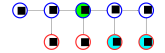
\includegraphics[scale=0.6]{ch2/beta_example.pdf}
\end{center}

\subsection{beta-4}
\begin{definition}[$\left | \beta_{t_4} \right > $]
As you can see in Definition(\ref{specialposterior}), we let
\begin{equation}\label{beta4}
        \left<x|\beta_{t_4} \right>=1~~\forall x 
\end{equation}
and we want to find $\left|\beta_{t_4} \right> $ which is in eigenspace
\begin{equation}
        \left|\beta_{t_4} \right> = \begin{bmatrix}
                \left< \psi_1|\beta_{t_4} \right> \\ \left< \psi_2|\beta_{t_4} \right> \\ \vdots \\ 
                \left< \psi_{72}|\beta_{t_4} \right>
        \end{bmatrix} 
\end{equation}
where
\begin{equation}\label{beta4dotproduct}
        \left< \psi_j | \beta_{t_4} \right> = \int w(x) \psi_j(x)  \left<x|\beta_{t_4} \right> dx
        = \int w(x) \psi_j(x) dx \approx \sum_{i=1}^{193} w(x_i) \psi_j(x_i).
\end{equation}
We substitute eq(\ref{beta4}) into eq(\ref{beta4dotproduct}).
\begin{center}
        \includegraphics[scale=0.45]{ch5/beta_t4.png}
\end{center}
\end{definition}

\subsection{beta-3}
\begin{definition}[$ \left| \beta_{t_3} \right>$]
\begin{equation}
        \left|\beta_{t_3}  \right> =  \left| e^{-\textbf{H}\Delta t} \textbf{y}_4 |\beta_{t_4} \right>
\end{equation}
The probability meaning is
\begin{equation}
   \left( \left<x_3 |\beta_{t_3}  \right> \right)^2 = p(y_4 | x_3) = \int p(x_4 | x_3) p(y_4 | x_4) dx_4
\end{equation}
\begin{center}
        \includegraphics[scale=0.6]{ch2/beta_3_graphical.pdf}
\end{center}
\begin{center}
        \includegraphics[scale=0.45]{ch5/beta_3.png}
\end{center}
\end{definition}

\begin{definition}[$\left| \hat{\beta}_{t_3} \right>$]
\begin{equation}
        \left| \hat{\beta}_{t_{3}} \right> = \frac{ \left| \beta_{t_{3}} \right> }{ c_4 }
\end{equation}
where $c_4$ is the scaling factor computed in the forward part, as you can see in eq(\ref{eq:scalefactor}), and 
the probability meaning is
\begin{equation}
        \left(\left<x_3|\hat{\beta}_{t_{3}} \right>\right)^2 = \frac{p(y_4|x_3)}{p(y_4|y_1,y_2,y_3)} 
        =  \frac{ (\left<x_3|\beta_{t_{3}} \right>)^2 }{ c_4^2 }
\end{equation}
\begin{center}
        \includegraphics[scale=0.45]{ch5/beta_3_hat.png}
\end{center}
\begin{equation}
        p(x_3|\textbf{y}) = (\left<\hat{\alpha}_{t_{3}}|x \right>)^2 \left(\left<x|\hat{\beta}_{t_{3}} \right>\right)^2
\end{equation} 
\end{definition}

\subsection{beta-2}
\begin{definition}[$\left| \beta_{t_2} \right>$]
\begin{equation}
        \left|\beta_{t_2}  \right> =  \left| e^{-\textbf{H}\Delta t} \textbf{y}_3 |\beta_{t_3} \right>
\end{equation}
The probability meaning is
\begin{equation}
           \left( \left<x_2 |\beta_{t_2}  \right> \right)^2 = p(y_3, y_4 | x_2)
\end{equation}
\begin{center}
        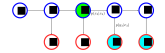
\includegraphics[scale=0.6]{ch2/beta_2_graphical.pdf}
\end{center}       
\end{definition}

\begin{definition}[$\left| \hat{\beta}_{t_2} \right>$]
\begin{equation}
        \left|\hat{\beta}_{t_2}  \right> =  \frac{\left| e^{-\textbf{H}\Delta t} \textbf{y}_3 |\hat{\beta}_{t_3} \right>}{c_3}
\end{equation}
where $c_3$ is the scaling factor computed in the forward part, as you can see in eq(\ref{eq:scalefactor}), and 
the probability meaning is
\begin{equation}
        \left(\left<x_2|\hat{\beta}_{t_{2}} \right>\right)^2 = \frac{p(y_3, y_4|x_2)}{p(y_3|y_1,y_2)} 
        =  \frac{ (\left<x_2|\beta_{t_{2}} \right>)^2 }{ c_3^2 }
\end{equation}
\begin{center}
        \includegraphics[scale=0.45]{ch5/beta_2_hat.png}
\end{center}
\begin{equation}
        p(x_2|\textbf{y}) = (\left<\hat{\alpha}_{t_{2}}|x \right>)^2 \left(\left<x|\hat{\beta}_{t_{2}} \right>\right)^2
\end{equation} 
\end{definition}

\subsection{beta-1}
\begin{definition}[$\left| \beta_{t_1} \right>$]
\begin{equation}
        \left|\beta_{t_1}  \right> =  \left| e^{-\textbf{H}\Delta t} \textbf{y}_2 |\beta_{t_2} \right>
\end{equation}
The probability meaning is
\begin{equation}
           \left( \left<x_1 |\beta_{t_1}  \right> \right)^2 = p(y_2, y_3, y_4 | x_1)
\end{equation}
\begin{center}
        \includegraphics[scale=0.6]{ch2/beta_1_graphical.pdf}
\end{center}       
\end{definition}

\begin{definition}[$\left| \hat{\beta}_{t_1} \right>$]
        \begin{equation}
                \left|\hat{\beta}_{t_1}  \right> =  \frac{\left| e^{-\textbf{H}\Delta t} \textbf{y}_2 |\hat{\beta}_{t_2} \right>}{c_2}
        \end{equation}
        where $c_2$ is the scaling factor computed in the forward part, as you can see in eq(\ref{eq:scalefactor}), and 
        the probability meaning is
        \begin{equation}
                \left(\left<x_1|\hat{\beta}_{t_1} \right>\right)^2 = \frac{p(y_2, y_3, y_4|x_1)}{p(y_2|y_1)} 
                =  \frac{ (\left<x_1|\beta_{t_1} \right>)^2 }{ c_2^2 }
        \end{equation}
        \begin{center}
                \includegraphics[scale=0.45]{ch5/beta_1_hat.png}
        \end{center}
        \begin{equation}
                p(x_1|\textbf{y}) = (\left<\hat{\alpha}_{t_{1}}|x \right>)^2 \left(\left<x|\hat{\beta}_{t_{1}} \right>\right)^2
        \end{equation} 
\end{definition}